\documentclass[12pt,a4paper]{article}
\usepackage[utf8]{vietnam}
\usepackage{amsmath,amssymb}
\usepackage{tabularx}
\usepackage{graphicx}
\usepackage{tikz}
\usetikzlibrary{calc,arrows.meta}
\usepackage{xcolor}
\usepackage{enumitem}
\usepackage{fancyhdr}
\usepackage[top=1.0cm, bottom=1.0cm, left=1.3cm, right=1.3cm]{geometry}
\usepackage[loigiai]{ex_test}
\SAOPTN{widthSA=2.6,heightSA=0.62}

\setlength{\headheight}{15pt}
\setlength{\parskip}{1pt}

\pagestyle{fancy}
\fancyhf{}
\rhead{\textit{Lời giải chi tiết -- Đề số 14}}
\lhead{\textit{Bộ đề ôn tập Giữa học kì I -- Toán 7}}
\cfoot{\thepage}

\begin{document}

\begin{center}
\textbf{\Large HƯỚNG DẪN CHẤM VÀ LỜI GIẢI CHI TIẾT}\\
\vspace{1mm}
\textbf{\large MÔN: TOÁN 7 -- ĐỀ SỐ 14}
\end{center}
\vspace{2mm}

\noindent\textbf{\large PHẦN I. CÂU TRẮC NGHIỆM NHIỀU PHƯƠNG ÁN LỰA CHỌN}

\vspace{1mm}
\begin{ex}
Phát biểu nào sau đây là đúng?
\choice
{$\sqrt{2} \in \mathbb{Q}$}
{$-5 \notin \mathbb{Q}$}
{$-\dfrac{5}{4} \notin \mathbb{Q}$}
{\True $\dfrac{3}{2} \in \mathbb{Q}$}
\loigiai{
Ta có $\dfrac{3}{2}$ là phân số có tử và mẫu là các số nguyên ($2 \neq 0$) nên $\dfrac{3}{2} \in \mathbb{Q}$.
}
\end{ex}

\begin{ex}
Số giá trị nguyên của $x$ thỏa mãn $-\dfrac{2}{3} < \dfrac{x}{12} < -\dfrac{1}{4}$ là:
\choice
{$3$}
{$2$}
{$5$}
{\True $4$}
\loigiai{
Quy đồng mẫu số chung 12: $-\dfrac{8}{12} < \dfrac{x}{12} < -\dfrac{3}{12} \iff -8 < x < -3$. Do $x \in \mathbb{Z}$ nên $x \in \{-7; -6; -5; -4\}$. Có 4 giá trị thỏa mãn.
}
\end{ex}

\begin{ex}
Số $9$ có căn bậc hai số học là:
\choice
{$3$ và $-3$}
{\True $3$}
{$-3$}
{$18$}
\loigiai{
Căn bậc hai số học của một số không âm $a$ là $\sqrt{a} \ge 0$. Do đó căn bậc hai số học của $9$ là $\sqrt{9} = 3$.
}
\end{ex}

\begin{ex}
\immini{
Cho hình vẽ bên, biết $OB$ là tia phân giác của $\widehat{AOC}$. Khi đó số đo của $\widehat{AOB}$ là:
\choice
{$65^\circ$}
{\True $32^\circ$}
{$130^\circ$}
{$18^\circ$}
}{
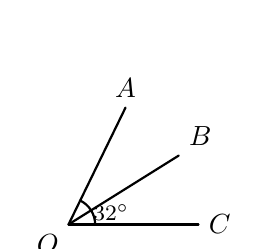
\begin{tikzpicture}[scale=0.75, line cap=round, line join=round]
    \coordinate (O) at (0,0);
    \coordinate (C) at (2.2,0);
    \coordinate (B) at (32:2.2);
    \coordinate (A) at (64:2.2);
    \draw[thick] (O) -- (C) node[right] {$C$};
    \draw[thick] (O) -- (B) node[above right] {$B$};
    \draw[thick] (O) -- (A) node[above] {$A$};
    \node[below left] at (O) {$O$};
    \draw[thick] (O) ++(0:0.45) arc (0:32:0.45);
    \node[font=\footnotesize] at (16:0.75) {$32^\circ$};
    \draw[thick] (O) ++(32:0.45) arc (32:64:0.45);
\end{tikzpicture}
}
\loigiai{
Do $OB$ là tia phân giác của $\widehat{AOC}$ nên $\widehat{AOB} = \widehat{BOC} = 32^\circ$.
}
\end{ex}

\begin{ex}
Kết quả của phép tính $\left(-\dfrac{1}{3}\right)^{2024} : \left(-\dfrac{1}{3}\right)^{2022}$ là:
\choice
{$\dfrac{1}{3}$}
{$-\dfrac{1}{9}$}
{\True $\dfrac{1}{9}$}
{$-\dfrac{2}{3}$}
\loigiai{
Áp dụng quy tắc chia hai lũy thừa cùng cơ số: $\left(-\dfrac{1}{3}\right)^{2024 - 2022} = \left(-\dfrac{1}{3}\right)^2 = \dfrac{1}{9}$.
}
\end{ex}

\begin{ex}
\immini{
Quan sát trục số bên dưới và chọn đáp án đúng về giá trị của điểm $a$:
\choice
{$a = \dfrac{1}{3}$}
{$a = \dfrac{1}{2}$}
{$a = \dfrac{2}{5}$}
{\True $a = \dfrac{2}{3}$}
}{
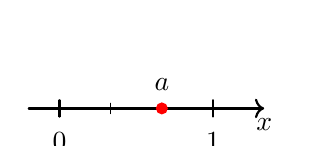
\begin{tikzpicture}[scale=1.3, line cap=round, line join=round]
    \draw[thick, ->] (-0.3,0) -- (2.0,0) node[below] {$x$};
    \draw[thick] (0, 0.08) -- (0, -0.08) node[below=2pt] {$0$};
    \draw[thick] (1.5, 0.08) -- (1.5, -0.08) node[below=2pt] {$1$};
    \draw (0.5, 0.05) -- (0.5, -0.05);
    \draw (1.0, 0.05) -- (1.0, -0.05);
    \filldraw[red] (1.0, 0) circle (1.5pt) node[above=3pt, black] {$a$};
\end{tikzpicture}
}
\loigiai{
Đoạn đơn vị từ $0$ đến $1$ được chia thành 3 phần bằng nhau. Điểm $a$ ở vạch chia thứ 2 theo chiều dương tính từ $0$, do đó $a = \dfrac{2}{3}$.
}
\end{ex}

\begin{ex}
Trong các số $\dfrac{9}{7}; 0{,}2; 0; -\dfrac{13}{5}; \dfrac{3}{15}; -\dfrac{2}{5}; -\dfrac{8}{5}$, có bao nhiêu số hữu tỉ dương?
\choice
{$1$}
{\True $3$}
{$2$}
{$4$}
\loigiai{
Các số hữu tỉ dương gồm có: $\dfrac{9}{7}; 0{,}2; \dfrac{3}{15}$ (tổng cộng 3 số).
}
\end{ex}

\begin{ex}
Cho $\widehat{xOy} = 80^\circ$. Góc đối đỉnh với $\widehat{xOy}$ có số đo độ là:
\choice
{$50^\circ$}
{\True $80^\circ$}
{$100^\circ$}
{$120^\circ$}
\loigiai{
Hai góc đối đỉnh thì bằng nhau nên góc đối đỉnh với $\widehat{xOy}$ cũng có số đo bằng $80^\circ$.
}
\end{ex}

\begin{ex}
Các mặt của hình lập phương đều là:
\choice
{\True Hình vuông}
{Tam giác đều}
{Hình chữ nhật}
{Hình thoi}
\loigiai{
Hình lập phương có 6 mặt đều là các hình vuông bằng nhau.
}
\end{ex}

\begin{ex}
\immini{
Cho hình vẽ bên, biết $\widehat{CFE} = 60^\circ, \widehat{E}_1 = 120^\circ$. Xét hai khẳng định: (I) $\widehat{BEF} = 60^\circ$; (II) $AB \parallel CD$. Khẳng định nào sau đây là đúng?
\choice
{Chỉ (I) đúng}
{Chỉ (II) đúng}
{\True Cả (I) và (II) đều đúng}
{Cả (I) và (II) đều sai}
}{
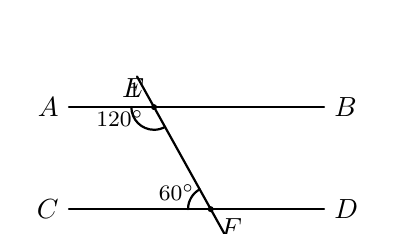
\begin{tikzpicture}[scale=0.72, line cap=round, line join=round]
    \draw[thick] (-2, 1.8) node[left] {$A$} -- (2.5, 1.8) node[right] {$B$};
    \draw[thick] (-2, 0) node[left] {$C$} -- (2.5, 0) node[right] {$D$};
    \coordinate (E) at (-0.5, 1.8);
    \coordinate (F) at (0.5, 0);
    \draw[thick] ($(E)!-0.3!(F)$) -- ($(F)!-0.3!(E)$);
    \filldraw[black] (E) circle (1.2pt) node[above left] {$E$};
    \filldraw[black] (F) circle (1.2pt) node[below right] {$F$};
    % E1 = 120 (angle AEF)
    \draw[thick] (E) ++(180:0.4) arc (180:299.1:0.4);
    \node[font=\footnotesize] at ($(E)+(-0.6,-0.2)$) {$120^\circ$};
    \node[font=\footnotesize] at ($(E)+(-0.35,0.3)$) {$1$};
    % CFE = 60
    \draw[thick] (F) ++(180:0.4) arc (180:119.1:0.4);
    \node[font=\footnotesize] at ($(F)+(-0.6,0.3)$) {$60^\circ$};
\end{tikzpicture}
}
\loigiai{
Vì $\widehat{BEF}$ và $\widehat{E}_1$ là hai góc kề bù nên $\widehat{BEF} = 180^\circ - 120^\circ = 60^\circ$ (khẳng định I đúng). Mặt khác, $\widehat{CFE} = \widehat{BEF} = 60^\circ$ là hai góc so le trong bằng nhau nên $AB \parallel CD$ (khẳng định II đúng).
}
\end{ex}

\begin{ex}
Hai đường thẳng $xx'$ và $yy'$ cắt nhau tại $O$. Góc đối đỉnh với $\widehat{x'Oy}$ là:
\choice
{\True $\widehat{xOy'}$}
{$\widehat{x'Oy}$}
{$\widehat{x'Oy'}$}
{$\widehat{xOy}$}
\loigiai{
Tia đối của $Ox'$ là $Ox$, của $Oy$ là $Oy'$. Vậy góc đối đỉnh với $\widehat{x'Oy}$ là $\widehat{xOy'}$.
}
\end{ex}

\begin{ex}
Cho ba đường thẳng phân biệt $a, b, c$ biết $a \parallel c$ và $b \parallel c$. Kết luận nào sau đây là đúng?
\choice
{$a$ cắt $b$}
{\True $a \parallel b$}
{$a \perp b$}
{$a$ trùng $b$}
\loigiai{
Hai đường thẳng phân biệt cùng song song với một đường thẳng thứ ba thì chúng song song với nhau ($a \parallel b$).
}
\end{ex}


\setcounter{ex}{0}
\noindent\textbf{\large PHẦN II. CÂU TRẮC NGHIỆM ĐÚNG SAI}

\vspace{1mm}
\begin{ex}
Cho biểu thức $P = \dfrac{3}{5} \cdot \left(-\dfrac{5}{6}\right) + \left(-\dfrac{1}{2}\right)^2 - \left|-\dfrac{3}{4}\right|$. Xét tính đúng sai của các mệnh đề sau:
\choiceTF
{\True Giá trị của phép nhân $\dfrac{3}{5} \cdot \left(-\dfrac{5}{6}\right)$ bằng $-\dfrac{1}{2}$}
{Giá trị của lũy thừa $\left(-\dfrac{1}{2}\right)^2$ bằng $-\dfrac{1}{4}$}
{\True Giá trị tuyệt đối $\left|-\dfrac{3}{4}\right|$ bằng $\dfrac{3}{4}$}
{\True Giá trị của biểu thức $P$ bằng $-1$}
\loigiai{
\begin{itemize}[leftmargin=0.6cm, itemsep=1pt]
\item \textbf{a)} \textbf{Đúng}. Ta có $\dfrac{3}{5} \cdot \left(-\dfrac{5}{6}\right) = -\dfrac{3 \cdot 5}{5 \cdot 6} = -\dfrac{3}{6} = -\dfrac{1}{2}$.
\item \textbf{b)} \textbf{Sai}. Ta có $\left(-\dfrac{1}{2}\right)^2 = \dfrac{(-1)^2}{2^2} = \dfrac{1}{4} \neq -\dfrac{1}{4}$.
\item \textbf{c)} \textbf{Đúng}. Giá trị tuyệt đối của một số luôn không âm nên $\left|-\dfrac{3}{4}\right| = \dfrac{3}{4}$.
\item \textbf{d)} \textbf{Đúng}. Thay các giá trị vào biểu thức: $P = -\dfrac{1}{2} + \dfrac{1}{4} - \dfrac{3}{4} = -\dfrac{2}{4} + \dfrac{1}{4} - \dfrac{3}{4} = -\dfrac{4}{4} = -1$.
\end{itemize}
}
\end{ex}

\begin{ex}
\immini{
Quan sát hình vẽ bên, biết đường thẳng $d \perp m$ tại $H$, $d \perp n$ tại $I$; đường thẳng $c$ cắt $m$ tại $A$ và cắt $n$ tại $B$ sao cho $\widehat{ABI} = 80^\circ$. Xét tính đúng sai của các mệnh đề sau:
\choiceTF
{\True Hai đường thẳng $m$ và $n$ song song với nhau ($m \parallel n$)}
{\True Góc so le trong với góc $\widehat{ABI}$ tại đỉnh $A$ có số đo bằng $80^\circ$}
{Góc trong cùng phía với góc $\widehat{ABI}$ tại đỉnh $A$ có số đo bằng $80^\circ$}
{\True Số đo góc $\widehat{AHI}$ bằng $90^\circ$}
}{
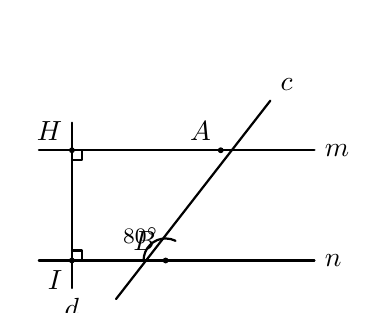
\begin{tikzpicture}[scale=0.7, line cap=round, line join=round]
    % Lines m and n
    \draw[thick] (-2.2, 2.0) -- (2.8, 2.0) node[right] {$m$};
    \draw[thick] (-2.2, 0) -- (2.8, 0) node[right] {$n$};
    % Line d perpendicular at H and I
    \draw[thick] (-1.6, 2.5) -- (-1.6, -0.5) node[below] {$d$};
    \filldraw[black] (-1.6, 2.0) circle (1.2pt) node[above left] {$H$};
    \filldraw[black] (-1.6, 0) circle (1.2pt) node[below left] {$I$};
    \draw[thick] (-1.6, 2.0) ++(0,-0.18) -- ++(0.18,0) -- ++(0,0.18);
    \draw[thick] (-1.6, 0) ++(0,0.18) -- ++(0.18,0) -- ++(0,-0.18);
    % Line c slanted cutting m at A, n at B
    \draw[thick] (2.0, 2.9) node[above right] {$c$} -- (-0.8, -0.7);
    \filldraw[black] (1.1, 2.0) circle (1.2pt) node[above left] {$A$};
    \filldraw[black] (0.1, 0) circle (1.2pt) node[above left] {$B$};
    % Angle ABI = 80
    \draw[thick] (0.1, 0) ++(180:0.4) arc (180:63.4:0.4);
    \node[font=\footnotesize] at (-0.35, 0.45) {$80^\circ$};
\end{tikzpicture}
}
\loigiai{
\begin{itemize}[leftmargin=0.6cm, itemsep=1pt]
\item \textbf{a)} \textbf{Đúng}. Vì $m \perp d$ và $n \perp d$ nên $m \parallel n$.
\item \textbf{b)} \textbf{Đúng}. Vì $m \parallel n$ nên góc so le trong với $\widehat{ABI}$ tại đỉnh $A$ bằng $\widehat{ABI} = 80^\circ$.
\item \textbf{c)} \textbf{Sai}. Hai góc trong cùng phía bù nhau, do đó góc trong cùng phía với $\widehat{ABI}$ có số đo bằng $180^\circ - 80^\circ = 100^\circ$ chứ không phải $80^\circ$.
\item \textbf{d)} \textbf{Đúng}. Vì $d \perp m$ tại $H$ nên $\widehat{AHI} = 90^\circ$.
\end{itemize}
}
\end{ex}


\setcounter{ex}{0}
\noindent\textbf{\large PHẦN III. CÂU HỎI TRẢ LỜI NGẮN}

\vspace{1mm}
\begin{ex}
Tìm số hữu tỉ $x$, biết: $3 \cdot \left(x - \dfrac{1}{4}\right) + \dfrac{1}{2} = \dfrac{1}{3}$. \shortans{$\dfrac{7}{36}$}
\loigiai{
Ta có: $3 \cdot \left(x - \dfrac{1}{4}\right) = \dfrac{1}{3} - \dfrac{1}{2} = -\dfrac{1}{6} \iff x - \dfrac{1}{4} = -\dfrac{1}{6} : 3 = -\dfrac{1}{18} \iff x = -\dfrac{1}{18} + \dfrac{1}{4} = \dfrac{-2 + 9}{36} = \dfrac{7}{36}$.

\textbf{Đáp số:} $\dfrac{7}{36}$
}
\end{ex}

\begin{ex}
\immini{
Cho hình hộp chữ nhật $ABCD.A'B'C'D'$ như hình vẽ có chiều dài $D'C' = 4\text{ cm}$, chiều rộng $B'C' = 2\text{ cm}$ và chiều cao $BB' = 3\text{ cm}$. Tính thể tích của hình hộp chữ nhật này.
\vspace{1mm}
\hfill\shortans{$24\text{ cm}^3$}
}{
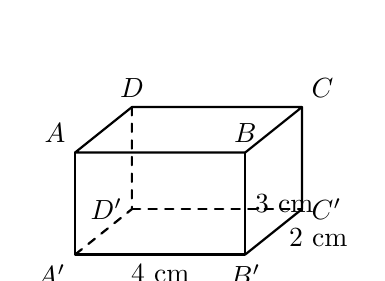
\begin{tikzpicture}[scale=0.72, line cap=round, line join=round]
    \coordinate (A) at (0, 1.8);
    \coordinate (B) at (3.0, 1.8);
    \coordinate (C) at (4.0, 2.6);
    \coordinate (D) at (1.0, 2.6);
    \coordinate (A_prime) at (0, 0);
    \coordinate (B_prime) at (3.0, 0);
    \coordinate (C_prime) at (4.0, 0.8);
    \coordinate (D_prime) at (1.0, 0.8);

    \draw[thick] (A) -- (B) -- (C) -- (D) -- cycle;
    \draw[thick] (A) -- (A_prime) -- (B_prime) -- (B);
    \draw[thick] (B_prime) -- (C_prime) -- (C);
    \draw[thick, dashed] (D) -- (D_prime) -- (A_prime);
    \draw[thick, dashed] (D_prime) -- (C_prime);

    \node[above left] at (A) {$A$};
    \node[above] at (B) {$B$};
    \node[above right] at (C) {$C$};
    \node[above] at (D) {$D$};
    \node[below left] at (A_prime) {$A'$};
    \node[below] at (B_prime) {$B'$};
    \node[right] at (C_prime) {$C'$};
    \node[left] at (D_prime) {$D'$};

    \node[below] at ($(A_prime)!0.5!(B_prime)$) {$4\text{ cm}$};
    \node[right] at ($(B_prime)!0.5!(C_prime)+(0.1,-0.1)$) {$2\text{ cm}$};
    \node[right] at ($(B)!0.5!(B_prime)$) {$3\text{ cm}$};
\end{tikzpicture}
}
\loigiai{
Thể tích của hình hộp chữ nhật là: $V = a \cdot b \cdot c = 4 \cdot 2 \cdot 3 = 24\text{ cm}^3$.

\textbf{Đáp số:} $24\text{ cm}^3$
}
\end{ex}


\setcounter{ex}{0}
\noindent\textbf{\large PHẦN IV. TỰ LUẬN}

\vspace{1mm}
\begin{ex}
Tính giá trị các biểu thức sau (tính bằng cách hợp lý nếu có thể):
\begin{enumerate}[label=\textbf{\alph*)}, leftmargin=0.8cm, itemsep=1pt]
\item $A = \dfrac{2}{7} + \left(-\dfrac{3}{7}\right) : \dfrac{3}{2}$
\item $B = \dfrac{5}{17} \cdot \left(-\dfrac{31}{33}\right) + \dfrac{5}{17} \cdot \left(-\dfrac{2}{33}\right) + 2\dfrac{5}{17}$
\item $C = \sqrt{4} + \sqrt{9} + \sqrt{16} + \sqrt{25}$
\item $D = 0{,}(5) - 1\dfrac{1}{3} - 0{,}(7)$
\end{enumerate}
\loigiai{
\textbf{a)} $A = \dfrac{2}{7} + \left(-\dfrac{3}{7}\right) \cdot \dfrac{2}{3} = \dfrac{2}{7} + \left(-\dfrac{2}{7}\right) = 0$.

\textbf{b)} $B = \dfrac{5}{17} \cdot \left(-\dfrac{31}{33} - \dfrac{2}{33}\right) + 2 + \dfrac{5}{17} = \dfrac{5}{17} \cdot (-1) + \dfrac{5}{17} + 2 = -\dfrac{5}{17} + \dfrac{5}{17} + 2 = 2$.

\textbf{c)} $C = 2 + 3 + 4 + 5 = 14$.

\textbf{d)} Đổi sang phân số: $0{,}(5) = \dfrac{5}{9}; 0{,}(7) = \dfrac{7}{9}; 1\dfrac{1}{3} = \dfrac{4}{3} = \dfrac{12}{9}$. Khi đó: $D = \dfrac{5}{9} - \dfrac{12}{9} - \dfrac{7}{9} = \dfrac{5 - 12 - 7}{9} = -\dfrac{14}{9}$.
}
\end{ex}
\vspace{2mm}

\begin{ex}
Tìm $x$, biết:
\begin{enumerate}[label=\textbf{\alph*)}, leftmargin=0.8cm, itemsep=1pt]
\item $2x - \dfrac{1}{3} = \dfrac{5}{6}$
\item $\left(x - \dfrac{1}{2}\right)^2 = \dfrac{9}{25}$
\end{enumerate}
\loigiai{
\textbf{a)} $2x = \dfrac{5}{6} + \dfrac{1}{3} = \dfrac{5}{6} + \dfrac{2}{6} = \dfrac{7}{6} \iff x = \dfrac{7}{6} : 2 = \dfrac{7}{12}$. Vậy $x = \dfrac{7}{12}$.

\textbf{b)} Vì $\left(\dfrac{3}{5}\right)^2 = \dfrac{9}{25}$ và $\left(-\dfrac{3}{5}\right)^2 = \dfrac{9}{25}$, ta xét hai trường hợp:\par $\bullet$ TH1: $x - \dfrac{1}{2} = \dfrac{3}{5} \iff x = \dfrac{3}{5} + \dfrac{1}{2} = \dfrac{6 + 5}{10} = \dfrac{11}{10}$.\par $\bullet$ TH2: $x - \dfrac{1}{2} = -\dfrac{3}{5} \iff x = -\dfrac{3}{5} + \dfrac{1}{2} = \dfrac{-6 + 5}{10} = -\dfrac{1}{10}$.\par Vậy $x = \dfrac{11}{10}$ hoặc $x = -\dfrac{1}{10}$.
}
\end{ex}
\vspace{2mm}

\begin{ex}
Bể cá của quán cà phê Koi có dạng hình hộp chữ nhật có chiều dài $1{,}8\text{ m}$, chiều rộng $1{,}2\text{ m}$ và chiều cao $1{,}5\text{ m}$.
\begin{enumerate}[label=\textbf{\alph*)}, leftmargin=0.8cm, itemsep=1pt]
\item Tính diện tích xung quanh của bể cá.
\item Chủ quán đã đổ nước vào bể sao cho mực nước cách miệng bể $20\text{ cm}$. Hỏi chủ quán đã đổ vào bể bao nhiêu lít nước? (biết rằng ban đầu bể không có nước).
\end{enumerate}
\loigiai{
\textbf{a)} Diện tích xung quanh của bể cá là: $S_{xq} = 2 \cdot (1{,}8 + 1{,}2) \cdot 1{,}5 = 2 \cdot 3 \cdot 1{,}5 = 9\text{ m}^2$.

\textbf{b)} Đổi $20\text{ cm} = 0{,}2\text{ m}$.\par Chiều cao mực nước trong bể là: $h = 1{,}5 - 0{,}2 = 1{,}3\text{ m}$.\par Thể tích nước đã đổ vào bể là: $V = 1{,}8 \cdot 1{,}2 \cdot 1{,}3 = 2{,}808\text{ m}^3$.\par Đổi $2{,}808\text{ m}^3 = 2808\text{ dm}^3 = 2808\text{ lít}$.\par Vậy chủ quán đã đổ vào bể $2808$ lít nước.
}
\end{ex}
\vspace{2mm}

\begin{ex}
Cho hai biểu thức sau: $A = \dfrac{25^{800} \cdot 16^{60} \cdot 3^{2500}}{8^{80} \cdot 27^{60} \cdot 5^{1600}}$ và $B = 3^{2025}$. Hãy so sánh $A$ và $B$.
\loigiai{
Ta có: $A = \dfrac{(5^2)^{800} \cdot (2^4)^{60} \cdot 3^{2500}}{(2^3)^{80} \cdot (3^3)^{60} \cdot 5^{1600}} = \dfrac{5^{1600} \cdot 2^{240} \cdot 3^{2500}}{2^{240} \cdot 3^{180} \cdot 5^{1600}}$.\par Rút gọn cả tử và mẫu cho $5^{1600}$ và $2^{240}$:\par \centerline{$A = \dfrac{3^{2500}}{3^{180}} = 3^{2500 - 180} = 3^{2320}$.}\par Vì $2320 > 2025$ nên $3^{2320} > 3^{2025} \implies A > B$.
}
\end{ex}
\vspace{2mm}


\begin{center}
\rule{4cm}{0.4pt}\\
\textit{--- HẾT ---}
\end{center}
\end{document}
